\documentclass[usepdftitle=false]{beamer}
% Set usepdftitle=false when \title{} contains complicated stuff.
% Author: alick<alick9188@gmail.com>
% 带中文支持的、使用 Beamer 的 NiuLab 幻灯片模板
% 使用 xelatex 编译

% This file is modified from a solution template for:

% - Giving a talk on some subject.
% - The talk is between 15min and 45min long.
% - Style is ornate.

% Copyright 2004 by Till Tantau <tantau@users.sourceforge.net>.
%
% In principle, this file can be redistributed and/or modified under
% the terms of the GNU Public License, version 2.
%
% However, this file is supposed to be a template to be modified
% for your own needs. For this reason, if you use this file as a
% template and not specifically distribute it as part of a another
% package/program, I grant the extra permission to freely copy and
% modify this file as you see fit and even to delete this copyright
% notice.

\mode<presentation>
{
\usetheme{niulab}
} % end of mode presentation

\usepackage{graphicx} % includegraphics support (already specified)
%\graphicspath{{fig/}} % directories that hold graphics
\usepackage{listings} % for typesetting source code
\usepackage{amsmath} % for math
\usepackage{siunitx} % for si units
\usepackage[style=ieee]{biblatex}
% NOTE: The sample bib file triggers a bug in biblatex-ieee regarding
% to multi-part page range.
% cf. https://github.com/josephwright/biblatex-ieee/issues/15

\usepackage{iftex}
\ifXeTeX
%% Begin xetex related configuration
%% Uncomment these lines to be able to use Chinese.
\usepackage{fontspec}
\usepackage[CJKchecksingle]{xeCJK}

% xeCJK conf setup
\punctstyle{kaiming}
\renewcommand\CJKfamilydefault{\CJKsfdefault} % for slides

\setCJKmainfont[BoldFont={WenQuanYi Micro Hei},
ItalicFont={AR PL UKai CN}]{AR PL UMing CN}
\setCJKsansfont{WenQuanYi Micro Hei}
\setCJKmonofont{WenQuanYi Micro Hei Mono}

\setCJKfamilyfont{zhsong}{AR PL UMing CN}
\setCJKfamilyfont{zhhei}{WenQuanYi Zen Hei}
\setCJKfamilyfont{zhkai}{AR PL UKai CN}

\newcommand*{\songti}{\CJKfamily{zhsong}} % 宋体
\newcommand*{\heiti}{\CJKfamily{zhhei}}   % 黑体
\newcommand*{\kaishu}{\CJKfamily{zhkai}}  % 楷书

\renewcommand\tablename{表格}

%% End xetex related configuration
\else
  \usepackage[utf8]{inputenc}
\fi

\title
{\textcolor{green!50!black}{GREEN} \alert{Wireless Communications}}
\hypersetup{pdftitle=GREEN Wireless Communications}

\author[short] % (optional, use only with lots of authors)
{Zhisheng NIU}

\def\niulab{%
\alert{N}etwork \alert{I}ntegration for \alert{U}biquitous %
\alert{L}inkage \alert{a}nd \alert{B}roadband%
(\alert{NiuLab})%
}

\institute[short] % (optional, but mostly needed)
{
\niulab\\
Tsinghua University, Beijing, China
}
% - Use the \inst command only if there are several affiliations.
% - Keep it simple, no one is interested in your street address.

%\date % (optional)
%{\today}
\date{}

%\subject{Talks}

\hypersetup{
pdfauthor={Zhisheng NIU},
pdfsubject={Talks},
pdfkeywords={GREEN,Wireless,Communications},
unicode=true,
}

% Delete this, if you do not want the table of contents to pop up at
% the beginning of each subsection:
%\AtBeginSubsection[]
%{
%  \begin{frame}<beamer>{Outline}
%    \tableofcontents[currentsection,currentsubsection]
%  \end{frame}
%}


% If you wish to uncover everything in a step-wise fashion, uncomment
% the following command:

%\beamerdefaultoverlayspecification{<+->}

% listings setup
\lstset{basicstyle=\ttfamily,breaklines=true}
% hyperref setup
\hypersetup{
%pdfpagemode=FullScreen,
}

\ExecuteBibliographyOptions{citetracker=true,sorting=none}

% Suppress publisher, location, note, etc. in citations.
\AtEveryCitekey{%
  %\ifentrytype{article}
    %{\clearfield{title}}
    %{}%
  \clearlist{publisher}%
  \clearlist{location}%
  \clearfield{isbn}%
  \clearfield{issn}%
  \clearfield{note}}

% Number of each bibliography entry in brackets
\DeclareFieldFormat{labelnumberwidth}{\mkbibbrackets{#1}}

\makeatletter
% Citation number in brackets.
\renewcommand\@makefntext[1]{%
  \normalfont[\@thefnmark]\enspace #1}
\makeatother

% Provide \notefullcite for footnote citations.
% cf. http://www.texdev.net/2010/03/08/biblatex-numbered-citations-as-footnotes/

% NOTE: for vanilla footnote coexistence, refer to
% http://tex.stackexchange.com/questions/20754/tuning-numbered-citations-as-footnote
% http://tex.stackexchange.com/questions/20787/biblatex-cite-with-footnote-only-once-with-use-of-brackets

\DeclareCiteCommand{\notefullcite}[\mkbibbrackets]
  {\usebibmacro{cite:init}%
   \usebibmacro{prenote}}
  {\usebibmacro{citeindex}%
   \usebibmacro{notefullcite}%
   \usebibmacro{cite:comp}}
  {}
  {\usebibmacro{cite:dump}%
   \usebibmacro{postnote}}

\newbibmacro*{notefullcite}{%
  \ifciteseen
    {}
    {\footnotetext[\thefield{labelnumber}]{%
       \usedriver{}{\thefield{entrytype}}.}}}

% Decrease the footnote size.
\let\oldfootnotesize\footnotesize
\renewcommand*{\footnotesize}{\oldfootnotesize\tiny}

\addbibresource{refs.bib}  % path to the bib database

% Disable the navigation symbol bar.
\beamertemplatenavigationsymbolsempty

\begin{document}

{
\usebackgroundtemplate{%
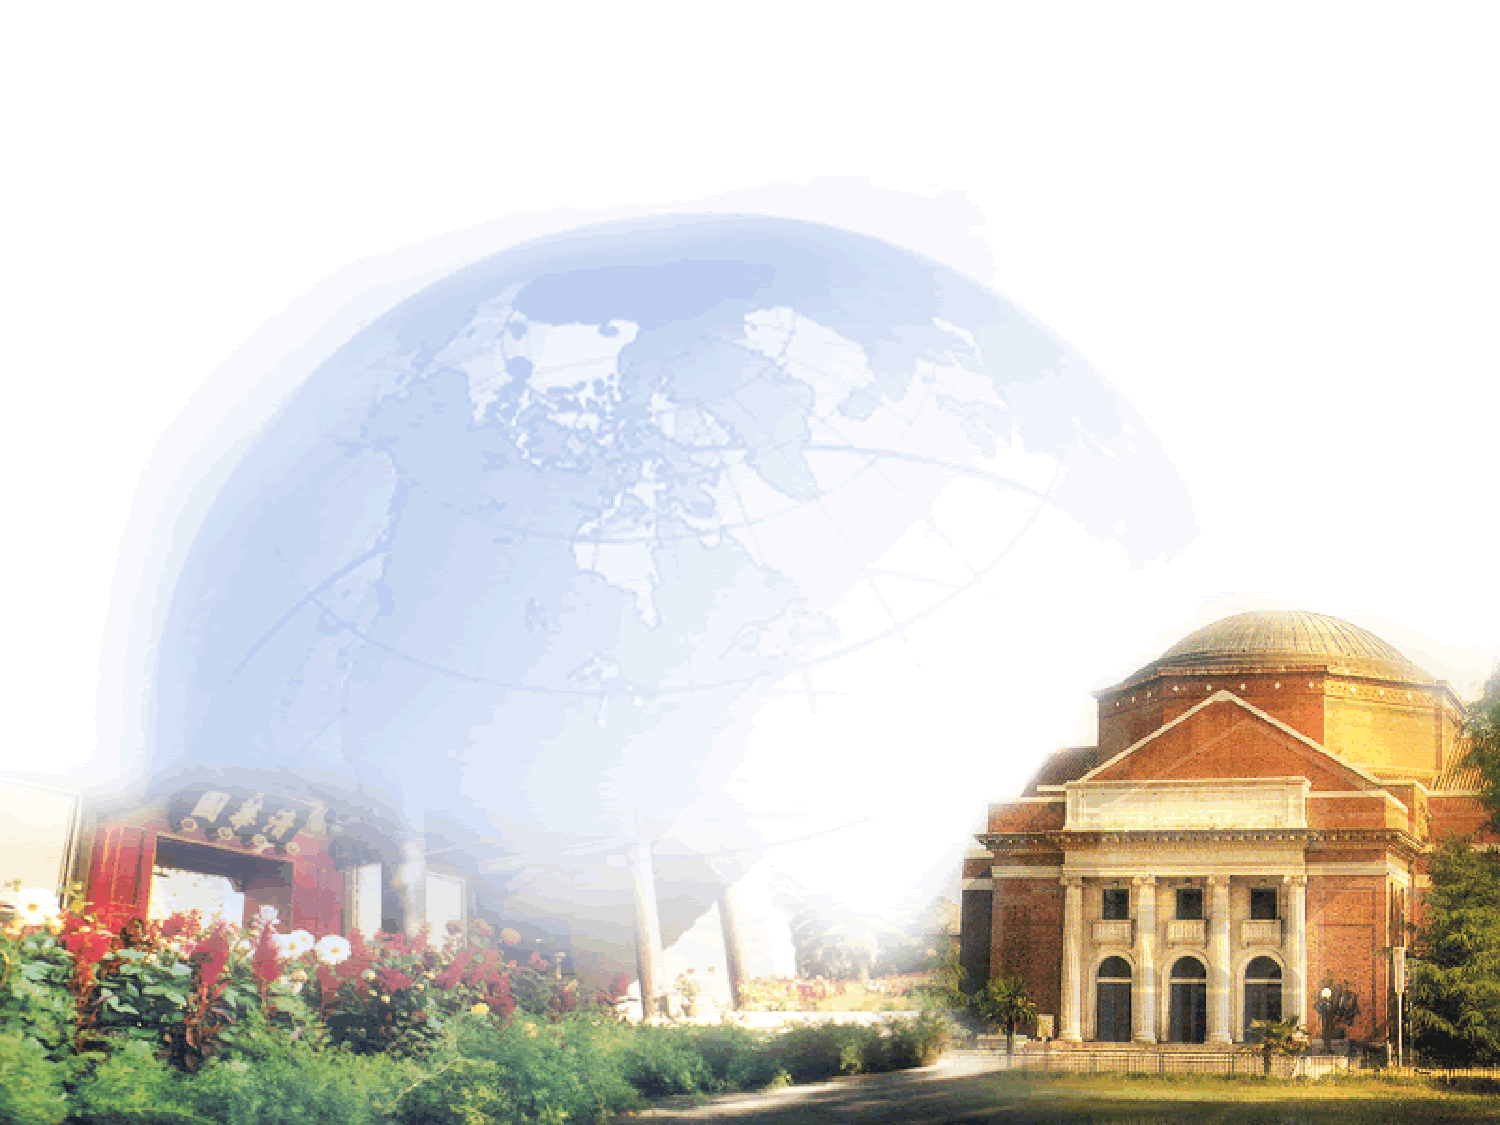
\includegraphics[width=\paperwidth,height=\paperheight]{niulab_titlepage_bg.pdf}}
\begin{frame}
\titlepage
\end{frame}
}

\begin{frame}{Contents}
\tableofcontents
% You might wish to add the option [pausesections]
\end{frame}


% Since this a solution template for a generic talk, very little can
% be said about how it should be structured. However, the talk length
% of between 15min and 45min and the theme suggest that you stick to
% the following rules:

% - Exactly two or three sections (other than the summary).
% - At *most* three subsections per section.
% - Talk about 30s to 2min per frame. So there should be between about
%   15 and 30 frames, all told.

\section{Information Technology in 2020}

\begin{frame}
  \frametitle{Computing Everywhere in 2020}
  \begin{itemize}
    \item Computers/computing everywhere --- $10^4$ CPUs per person
      \begin{itemize}
        \item Real-world computing --- sensors and actuators
        \item Massively distributed and embedded
        \item Collect data and make decisions
      \end{itemize}
    \item Massive data --- a TeraByte per person per day
      \begin{itemize}
        \item Sensors, personal, scientific, business, etc\ldots
        \item Extract information from this mass of data
        \item Serious privacy issues
      \end{itemize}
    \item People will spend much time in virtual environments
      \begin{itemize}
        \item Integrating digital and physical worlds
        \item Games, Interactive Movies, Virtual Classrooms --- many connected
        to physical spaces
      \end{itemize}
  \end{itemize}
\end{frame}

% TODO:
% Can blocks have transparent background?
%\begin{frame}
%  \frametitle{A Block Example}
%  \begin{block}{Computers/computing everywhere --- $10^4$ CPUs per person}
%    \begin{itemize}
%      \item Real-world computing --- sensors and actuators
%      \item Massively distributed and embedded
%      \item Collect data and make decisions
%    \end{itemize}
%  \end{block}
%\end{frame}


%\begin{frame}{Picture}
%  \begin{figure}[h]
%    \centering
%    \includegraphics[scale=0.4]{foo.png}
%    \caption{}
%  \end{figure}
%\end{frame}

\begin{frame}{Formulars}
  \begin{itemize}
    \item Electromagnetic Wave
      \begin{itemize}
        \item Maxwell:
          \begin{eqnarray*}
            \nabla \times \mathbf{E} & = & - \frac{\partial
            \mathbf{B}}{\partial t}\\
            \nabla \times \mathbf{H} & = & \mathbf{J} +
            \frac{\partial \mathbf{D}}{\partial t}\\
            \nabla \cdot \mathbf{D} & = & \rho \\
            \nabla \cdot\mathbf{B} & = & 0
            \label{maxwell}
          \end{eqnarray*}
      \end{itemize}
    \item Probability
      \begin{itemize}
        \item Normal Distribution $\mathcal{N}(\mu,\sigma^2)$:
          \[
          \int_{-\infty}^{\infty}\frac{1}{\sigma\sqrt{2\pi}}\mathrm{e}^{-\frac{(x-\mu)^2}{2\sigma^2}}\mathrm{d}x= 1 \, .
          \]
      \end{itemize}
  \end{itemize}
\end{frame}

\begin{frame}
  \frametitle{Title}
  \framesubtitle{Subtitle}
  \begin{itemize}
    \item item 1
    \item item 2
    \item Footnote citations~\notefullcite{beameruserguide,shannon1948}
  \end{itemize}
\end{frame}

\section{Vision and Mission of \protect\alert{NiuLab}}
\section{Current Major Research Topics}
\subsection{Multi-AP Diversity for Interference Avoidance}
\subsection{Cooperative Diversity for Opportunistic Scheduling}
\subsection{Integrated Communication and Broadcast NW for Data-casting
and Soft Realtime Services}
\subsection{\protect\alert{GREEN}: %
\protect\alert{G}lobally \protect\alert{R}esource-optimized \& %
\protect\alert{E}nergy-\protect\alert{E}fficient \protect\alert{N}W}

\section{Summary}

\begin{frame}{Summary}
  \begin{itemize}
    \item Blah...
  \end{itemize}
\end{frame}

\appendix
\section<presentation>*{\appendixname}

% Final logo page.
{
\usebackgroundtemplate{%

\includegraphics[width=\paperwidth,height=\paperheight]{niulab_logopage.pdf}}
\begin{frame}
\end{frame}
}
\end{document}
%%% vim: set sw=2 isk+=\: et tw=70 formatoptions+=mM:
